\documentclass[12pt]{article}
\usepackage[a4paper,margin=1.25cm]{geometry}
\usepackage{amsmath,amssymb,mathtools}
\usepackage{graphicx}
\usepackage{booktabs}
\usepackage{tabularx}
\usepackage{tikz}
\usepackage[T1]{fontenc}
\usepackage[utf8]{inputenc}
\usepackage[english]{babel}

\setlength{\parindent}{0pt}
\setlength{\parskip}{0.45em}
\setlength{\abovedisplayskip}{5pt plus 1pt minus 1pt}
\setlength{\belowdisplayskip}{5pt plus 1pt minus 1pt}
\setlength{\abovedisplayshortskip}{3pt plus 1pt minus 1pt}
\setlength{\belowdisplayshortskip}{3pt plus 1pt minus 1pt}

\newcommand{\dd}{\,\mathrm{d}}
\newcommand{\e}{\mathrm{e}}
\newcommand{\LL}{\lambda}

\begin{document}

\begin{center}
{\Large\bfseries The threshold \(a=\mathrm e\) for \((x-1)a^x+1\ge x^a\)}\\[0.35em]
{\large monotonicity, a double contact at \(x=0\) and \(x=1\), and two one-sided proofs}
\end{center}

\textbf{Problem.} Let \(a>1\) and
\[
f(x)=(x-1)a^x+1 .
\]
\begin{enumerate}
\item[(i)] For \(a>\e\), determine the intervals of monotonicity of \(f\).
\item[(ii)] Find all \(a>1\) for which
\[
(x-1)a^x+1\ge x^a\qquad\text{for every }x\ge0 .
\]
\end{enumerate}

\[
\boxed{\displaystyle
\text{(i)}\quad
f\downarrow\text{ on }(-\infty,x_0),\quad f\uparrow\text{ on }(x_0,\infty),
\quad x_0=1-\frac1{\log a};
\qquad
\text{(ii)}\quad 1<a\le\e .}
\]

\textbf{Overview.}
Throughout put
\[
\LL=\log a,\qquad a=\e^{\LL},
\]
which turns the threshold \(a=\e\) into \(\LL=1\). Part (i) is a
one-line derivative computation: the exponential factor is positive, so
the sign of \(f'\) is the sign of a linear function.

Part (ii) is governed by the difference
\[
F(x)=1+(x-1)\e^{\LL x}-x^{\e^{\LL}},
\]
which vanishes at \emph{two} points, \(x=0\) and \(x=1\). The necessity
of \(a\le\e\) is read off the slope at \(x=0\), where
\(F(x)\sim(1-\LL)x\). Sufficiency splits at the second contact point:
on \((0,1)\) a logarithmic-derivative comparison gives \(g(x)\ge x^a\)
directly, and on \([1,\infty)\) one shows \(F'\ge0\), so \(F\) grows away
from \(F(1)=0\). The point \(x=1\) is not an arbitrary cut: it is where
the two curves touch a second time.

\section*{1. Part (i): monotonicity}

Differentiating,
\[
f'(x)=a^x+(x-1)a^x\log a=a^x\bigl(1+(x-1)\log a\bigr).
\tag{1}
\]
Since \(a^x>0\) for all real \(x\), the sign of \(f'\) is the sign of the
affine factor \(1+(x-1)\log a\), which is increasing in \(x\) and
vanishes at
\[
x_0=1-\frac1{\log a}.
\tag{2}
\]
If \(a>\e\) then \(\log a>1\), so \(0<\frac1{\log a}<1\) and
\[
0<x_0<1 .
\]
Hence
\[
\boxed{\displaystyle
f'<0\ \text{on}\ (-\infty,x_0),\qquad
f'>0\ \text{on}\ (x_0,\infty),\qquad
x_0=1-\frac1{\log a}.}
\]
Restricted to \(x\ge0\), which is the range relevant to part (ii),
\(f\) decreases on \([0,x_0]\) and increases on \([x_0,\infty)\).

For \(1<a\le\e\) the same computation gives \(x_0\le0\), so \(f\) is
increasing on the whole of \([0,\infty)\). This fact reappears in
Section 4 as the positivity of \(g'\).

\section*{2. The two contact points}

Set
\[
F(x)=f(x)-x^a=1+(x-1)\e^{\LL x}-x^{\e^{\LL}},\qquad x\ge0 .
\]
Part (ii) asks for which \(\LL>0\) we have \(F\ge0\) on \([0,\infty)\).
Immediately
\[
F(0)=1-1-0=0,
\qquad
F(1)=1+0-1=0,
\tag{3}
\]
using \(a>1\) for \(0^a=0\). So the graph of \(f\) meets the graph of
\(x^a\) at both \(x=0\) and \(x=1\), and \(F\) must not dip below zero
between or beyond them. Any such problem is decided by local behaviour at
the contact points, and the softer of the two is \(x=0\).

\begin{center}
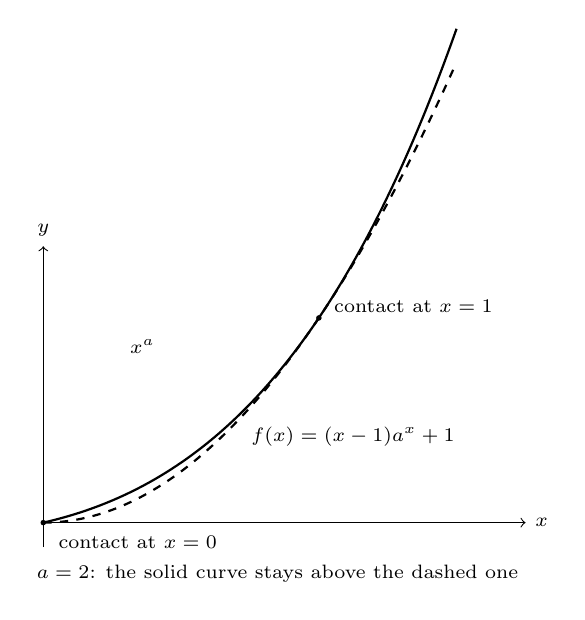
\begin{tikzpicture}[x=3.5cm,y=2.6cm]
\draw[->] (0,0)--(1.75,0) node[right] {\scriptsize \(x\)};
\draw[->] (0,-0.12)--(0,1.35) node[above] {\scriptsize \(y\)};
\draw[thick,samples=140,domain=0:1.5,smooth]
  plot (\x,{1+(\x-1)*exp(0.6931*\x)});
\draw[thick,dashed,samples=140,domain=0:1.5,smooth]
  plot (\x,{pow(\x,2)});
\fill (0,0) circle (1.0pt);
\fill (1,0.9999) circle (1.0pt);
\node[anchor=south west] at (1.02,0.98) {\scriptsize contact at \(x=1\)};
\node[anchor=north west] at (0.02,-0.02) {\scriptsize contact at \(x=0\)};
\node[anchor=west] at (0.72,0.42) {\scriptsize \(f(x)=(x-1)a^x+1\)};
\node[anchor=west] at (0.28,0.86) {\scriptsize \(x^a\)};
\node[anchor=north] at (0.85,-0.16) {\scriptsize \(a=2\): the solid curve stays above the dashed one};
\end{tikzpicture}
\end{center}

\section*{3. Necessity of \(a\le\mathrm e\)}

Expand near \(x=0^+\). Since \(\e^{\LL x}=1+\LL x+O(x^2)\),
\[
1+(x-1)\e^{\LL x}
=1+(x-1)\bigl(1+\LL x+O(x^2)\bigr)
=(1-\LL)x+O(x^2).
\tag{4}
\]
Moreover \(a>1\) gives \(x^a=o(x)\) as \(x\to0^+\). Hence
\[
\frac{F(x)}{x}\longrightarrow 1-\LL,\qquad x\to0^+ .
\tag{5}
\]
If \(\LL>1\), then \(1-\LL<0\), so \(F(x)<0\) for all sufficiently small
\(x>0\) and the inequality fails. Therefore
\[
\boxed{\LL\le1,\qquad\text{i.e.}\qquad 1<a\le\e .}
\tag{6}
\]

At the borderline \(\LL=1\) the linear term in (4) vanishes and
\[
1+(x-1)\e^{x}=\frac{x^2}{2}+\frac{x^3}{3}+\cdots,
\]
while \(x^{a}=x^{\e}\) with \(\e>2\), so \(x^{\e}=o(x^2)\) and
\(F(x)\sim\frac{x^2}{2}>0\). The threshold is thus decided by a
comparison of \emph{orders}: at \(a=\e\) the quadratic term saves the
inequality, and the exponent \(\e>2\) of the competing power is exactly
what makes it lose.

\section*{4. Sufficiency on \(0<x<1\)}

Assume \(0<\LL\le1\) and set
\[
g(x)=1+(x-1)\e^{\LL x}=1-(1-x)\e^{\LL x},
\]
so that \(F=g-x^a\) and the claim is \(g(x)\ge x^a\).

\textbf{Positivity of \(g\).} By (1) with \(f=g\),
\[
g'(x)=\e^{\LL x}\bigl(1-\LL(1-x)\bigr)\ge0
\qquad\text{for }0\le x\le1,
\tag{7}
\]
because \(\LL(1-x)\le\LL\le1\). Since \(g(0)=0\) and \(g(1)=1\), the
function \(g\) increases from \(0\) to \(1\) on \([0,1]\); in particular
\(g>0\) on \((0,1]\).

\textbf{The comparison of logarithmic derivatives.} We claim
\[
\frac{x\,g'(x)}{g(x)}\le a\qquad\text{for }0<x<1 .
\tag{8}
\]
Granting (8), divide by \(x>0\) and integrate over \([x,1]\):
\[
\int_x^1\frac{g'(t)}{g(t)}\dd t\le\int_x^1\frac{a}{t}\dd t .
\]
The left side is \(\log g(1)-\log g(x)=-\log g(x)\) since \(g(1)=1\); the
right side is \(-a\log x\). Hence \(\log g(x)\ge a\log x\) and,
exponentiating,
\[
g(x)\ge x^a,\qquad 0<x<1 .
\tag{9}
\]
This is the natural form of the argument: \(x^a\) is characterised by
having logarithmic derivative exactly \(\frac ax\), so (8) says that
\(g\) grows no faster than \(x^a\) on the way \emph{up} to the common
value \(1\) at \(x=1\), and therefore lies above it on the way
\emph{down}.

\textbf{Proof of (8).} Since \(x>0\) and \(g(x)>0\), (8) is equivalent to
\[
a\,g(x)-x\,g'(x)\ge0 .
\]
Substituting \(a=\e^{\LL}\) and (7), and putting \(y=1-x\in(0,1)\),
\[
\begin{aligned}
a\,g(x)-x\,g'(x)
&=\e^{\LL}\bigl(1-y\,\e^{\LL x}\bigr)-(1-y)\e^{\LL x}\bigl(1-\LL y\bigr)\\
&=\e^{\LL}\e^{-\LL y}\Bigl[\e^{\LL y}-\e^{\LL}y-(1-y)(1-\LL y)\Bigr]
=\e^{\LL x}H(y),
\end{aligned}
\]
where
\[
H(y):=\e^{\LL y}-\e^{\LL}y-(1-y)(1-\LL y).
\tag{10}
\]
It remains to prove \(H\ge0\) on \([0,1]\). Expanding both exponentials
and cancelling,
\[
H(y)=\LL y(1-y)-\sum_{n\ge2}\frac{\LL^n\bigl(y-y^n\bigr)}{n!} .
\tag{11}
\]
For \(0\le y\le1\),
\[
y-y^n=y(1-y)\bigl(1+y+\cdots+y^{n-2}\bigr)\le(n-1)\,y(1-y),
\]
so
\[
H(y)\ge y(1-y)\left[\LL-\sum_{n\ge2}\frac{(n-1)\LL^n}{n!}\right].
\tag{12}
\]
The series is elementary:
\[
\sum_{n\ge2}\frac{(n-1)\LL^n}{n!}
=\sum_{n\ge2}\left[\frac{\LL^n}{(n-1)!}-\frac{\LL^n}{n!}\right]
=\LL\bigl(\e^{\LL}-1\bigr)-\bigl(\e^{\LL}-1-\LL\bigr)
=(\LL-1)\e^{\LL}+1 .
\]
Therefore the bracket in (12) equals
\[
\LL-(\LL-1)\e^{\LL}-1=(1-\LL)\bigl(\e^{\LL}-1\bigr)\ge0
\qquad\text{for }0<\LL\le1,
\]
so \(H\ge0\), which proves (8) and hence (9):
\[
\boxed{F(x)\ge0\qquad(0<x<1).}
\]
Note where the hypothesis is used: the bracket is \((1-\LL)(\e^{\LL}-1)\),
which changes sign exactly at \(\LL=1\). The threshold of part (ii) is
visible a second time, now in the interior estimate.

\section*{5. Sufficiency on \(x\ge1\)}

Here it is cleanest to show that \(F\) is increasing, so that it never
returns below \(F(1)=0\). Differentiating and putting \(u=x-1\ge0\),
\[
F'(x)=\e^{\LL x}\bigl(1+\LL(x-1)\bigr)-a\,x^{a-1}
=\e^{\LL}\Bigl[\e^{\LL u}(1+\LL u)-(1+u)^{\e^{\LL}-1}\Bigr].
\]
Since \(\e^{\LL}>0\), it suffices that
\[
\e^{\LL u}(1+\LL u)\ge(1+u)^{\e^{\LL}-1},
\]
and both sides are positive, so we may take logarithms. Define
\[
R(u)=\LL u+\log(1+\LL u)-\bigl(\e^{\LL}-1\bigr)\log(1+u),
\qquad R(0)=0 .
\]
It suffices to prove \(R\ge0\) on \([0,\infty)\), and for that it suffices
that \(R'\ge0\). Now
\[
R'(u)=\LL+\frac{\LL}{1+\LL u}-\frac{\e^{\LL}-1}{1+u}
=\LL\left(1+\frac1{1+\LL u}\right)-\frac{\e^{\LL}-1}{1+u}.
\tag{13}
\]
Two elementary estimates finish the argument.

\textbf{Estimate A.} For \(u\ge0\) and \(0<\LL\le1\),
\[
1+\frac1{1+\LL u}\ge\frac2{1+u},
\]
because
\[
1+\frac1{1+\LL u}-\frac2{1+u}
=\frac{u\bigl(2-\LL+\LL u\bigr)}{(1+\LL u)(1+u)}\ge0 .
\]

\textbf{Estimate B.} For \(0\le\LL\le1\),
\[
\e^{\LL}-1\le2\LL .
\]
Indeed \(\psi(\LL)=1+2\LL-\e^{\LL}\) satisfies
\(\psi''(\LL)=-\e^{\LL}<0\), so \(\psi\) is concave; since
\(\psi(0)=0\) and \(\psi(1)=3-\e>0\), concavity puts \(\psi\) above the
chord joining these values, hence \(\psi\ge0\) on \([0,1]\).

Substituting A and B into (13),
\[
R'(u)\ge\frac{2\LL}{1+u}-\frac{\e^{\LL}-1}{1+u}
=\frac{2\LL-\bigl(\e^{\LL}-1\bigr)}{1+u}\ge0 .
\]
Therefore \(R\) is non-decreasing with \(R(0)=0\), so \(R\ge0\),
so \(F'\ge0\) on \([1,\infty)\), and with \(F(1)=0\),
\[
\boxed{F(x)\ge0\qquad(x\ge1).}
\]

\section*{6. Conclusion}

For \(0<\LL\le1\), that is \(1<a\le\e\), Sections 4 and 5 together with
(3) give
\[
F(0)=0,\qquad F\ge0\text{ on }(0,1),\qquad F(1)=0,\qquad F\ge0\text{ on }[1,\infty),
\]
so the inequality holds on all of \([0,\infty)\). Section 3 shows it
fails for \(a>\e\). Hence
\[
\boxed{\displaystyle
(x-1)a^x+1\ge x^a\ \text{ for all }x\ge0
\iff
1<a\le\e .}
\]

\section*{7. Numerical picture of the threshold}

Values of \(F(x)=1+(x-1)a^x-x^a\):

\begin{center}
\small
\renewcommand{\arraystretch}{1.3}
\begin{tabularx}{0.86\textwidth}{@{}lXXX@{}}
\toprule
\(x\) & \(a=2\) & \(a=\e\) & \(a=3\) \\
\midrule
\(0.01\) & \(0.003014\)  & \(0.0000467\) & \(-0.000937\) \\
\(0.05\) & \(0.013998\)  & \(0.001002\)  & \(-0.003769\) \\
\(0.10\) & \(0.025404\)  & \(0.003433\)  & \(-0.005511\) \\
\(0.20\) & \(0.041041\)  & \(0.010288\)  & \(-0.004585\) \\
\(0.50\) & \(0.042893\)  & \(0.023684\)  & \(\phantom{-}0.008975\) \\
\(1.00\) & \(0\)         & \(0\)         & \(0\) \\
\(2.00\) & \(1.000000\)  & \(1.808170\)  & \(\phantom{-}2.000000\) \\
\bottomrule
\end{tabularx}
\end{center}

For \(a=2<\e\) the values are comfortably positive; at \(a=\e\) they are
positive but tiny near the origin, consistent with \(F\sim\frac{x^2}{2}\)
from Section 3; for \(a=3>\e\) a genuine dip appears immediately to the
right of \(0\) and closes only near \(x\approx0.4\), matching
\(F(x)\sim(1-\log3)x\) with \(1-\log3=-0.0986\).

\section*{8. Remarks on the structure}

The computations are routine; the choice of structure is not.

\textbf{Where the threshold lives.} It is determined entirely at
\(x=0^+\), by the linear coefficient \(1-\log a\) in (4). Everything
after Section 3 is the verification that this necessary condition is also
sufficient, which is not automatic: \(F\) has a second zero at
\(x=1\) where it could in principle cross.

\textbf{Why cut at \(x=1\).} Because that is the second contact point.
Equivalently, the inequality \(1+(x-1)a^x\ge x^a\) can be rewritten, for
\(x\ne1\), as a comparison involving
\[
\frac{x^a-1}{x-1},
\]
the slope of the secant of \(t\mapsto t^a\) through \(t=1\). The
substitutions \(y=1-x\) in Section 4 and \(u=x-1\) in Section 5 both
recentre at that point, which is why each side yields a function
vanishing at the origin with a sign-definite derivative.

\textbf{Two different mechanisms on the two sides.} On \((0,1)\) the
direct approach through \(F'\) is awkward, because \(F\) starts and ends
at \(0\) and so \(F'\) must change sign; instead one compares logarithmic
derivatives, which is the right tool for showing that one function
dominates a pure power. On \([1,\infty)\) no such subtlety arises: \(F\)
starts at \(0\) and is shown to be non-decreasing outright. Attempting a
single uniform argument on \([0,\infty)\) is possible but produces a
quotient of exponentials with a quadratic numerator, and hides the role
of the double contact.

\end{document}
